% shared preamble of the theory figures (white background, purple / black theme, sans-serif)
\documentclass[tikz,border=8pt]{standalone}
\usepackage[T1]{fontenc}
\usepackage[scaled=0.92]{helvet}
\renewcommand{\familydefault}{\sfdefault}
\usepackage{amsmath,amssymb}
\usepackage[helvet]{sfmath}
\usetikzlibrary{arrows.meta,calc,decorations.pathreplacing,positioning,backgrounds}
\definecolor{ink}{HTML}{1A1A1F}
\definecolor{cohesin}{HTML}{6A3DE8}
\definecolor{condensin}{HTML}{1BAF7A}
\definecolor{fwd}{HTML}{D1303F}      % CTCF pointing right
\definecolor{rev}{HTML}{2B62D9}      % CTCF pointing left
\definecolor{panel}{HTML}{F8F6FD}
\definecolor{panelline}{HTML}{E3DDF5}
\tikzset{
  fiber/.style={line width=2.1pt,ink,line cap=round,line join=round},
  halo/.style={line width=6pt,white,line cap=round},
  lab/.style={font=\small,text=ink},
  note/.style={font=\footnotesize,text=ink!60},
  hd/.style={font=\bfseries\small,text=ink,anchor=west},
  leader/.style={line width=0.6pt,ink!45},
}
% soft panel, numbered badge, heading
\newcommand{\panelbg}[4]{\draw[rounded corners=9pt,fill=panel,draw=panelline,line width=0.9pt] (#1,#2) rectangle (#3,#4);}
\newcommand{\badge}[3]{\fill[ink] (#1,#2) circle (0.21);\node[white,font=\bfseries\footnotesize] at (#1,#2) {#3};}
% CTCF: a protein on the fibre carrying an arrow that gives the motif direction (f = right, r = left)
\newcommand{\protf}[2]{\draw[rounded corners=3.5pt,line width=0.6pt,draw=fwd!65!black,fill=fwd] (#1-0.3,#2-0.19) rectangle (#1+0.3,#2+0.19);
  \draw[white,line width=1.5pt,-{Stealth[length=3.4pt,width=4.4pt]}] (#1-0.15,#2)--(#1+0.16,#2);}
\newcommand{\protr}[2]{\draw[rounded corners=3.5pt,line width=0.6pt,draw=rev!65!black,fill=rev] (#1-0.3,#2-0.19) rectangle (#1+0.3,#2+0.19);
  \draw[white,line width=1.5pt,-{Stealth[length=3.4pt,width=4.4pt]}] (#1+0.15,#2)--(#1-0.16,#2);}
\newcommand{\prot}[3]{\csname prot#3\endcsname{#1}{#2}}
% ring seen at an angle, drawn as a tube (dark outline, light core); back half and front half
\newcommand{\ringpart}[5]{\draw[line width=4.6pt,#3!80!black,line cap=round] ([shift={(#1,#2)}]#4:0.55 and 0.21) arc[start angle=#4,end angle=#5,x radius=0.55,y radius=0.21];
  \draw[line width=2.4pt,#3!55!white,line cap=round] ([shift={(#1,#2)}]#4:0.55 and 0.21) arc[start angle=#4,end angle=#5,x radius=0.55,y radius=0.21];}
\newcommand{\ringback}[3]{\ringpart{#1}{#2}{#3}{180}{0}}
\newcommand{\ringfront}[3]{\ringpart{#1}{#2}{#3}{180}{360}}
% smooth loop whose foot (ring) is at (cx,y0): half-width W, height H, ring colour
\newcommand{\lloop}[5]{%
  \ringback{#1}{#2}{#5}%
  \draw[fiber] (#1-0.3,#2) .. controls (#1-0.3,#2+0.25*#4) and (#1-#3,#2+0.2*#4) .. (#1-#3,#2+0.55*#4)
     .. controls (#1-#3,#2+0.95*#4) and (#1-0.5*#3,#2+#4) .. (#1,#2+#4)
     .. controls (#1+0.5*#3,#2+#4) and (#1+#3,#2+0.95*#4) .. (#1+#3,#2+0.55*#4)
     .. controls (#1+#3,#2+0.2*#4) and (#1+0.3,#2+0.25*#4) .. (#1+0.3,#2);%
  \ringfront{#1}{#2}{#5}}
% gently undulating fibre from x0 to the loop foot at cx (height y0), and from x1
\newcommand{\base}[4]{%
  \draw[fiber] plot[smooth] coordinates {(#1,0.05) (#1+0.35*#3-0.35*#1,-0.05) (#3-1.4,0.04)} .. controls (#3-0.6,0.02) and (#3-0.3,0.05) .. (#3-0.3,#4);
  \draw[fiber] plot[smooth] coordinates {(#2,-0.05) (#2-0.35*#2+0.35*#3,0.05) (#3+1.4,-0.04)} .. controls (#3+0.6,-0.02) and (#3+0.3,0.05) .. (#3+0.3,#4);}
% stop sign for a blocked leg and a leg arrow
\newcommand{\stopbar}[3]{\draw[#3,line width=2.4pt,line cap=round] (#1,#2-0.2)--(#1,#2+0.2);}
\newcommand{\legarrow}[3]{\draw[cohesin,line width=1.6pt,-{Stealth[length=5pt,width=6pt]},line cap=round] (#1,#3)--(#2,#3);}

\tikzset{cA/.style={line width=2.6pt,cohesin,line cap=round},cB/.style={line width=2.6pt,ink,line cap=round},h/.style={line width=7pt,white,line cap=butt},
  st/.style={line width=2.6pt,ink,line cap=round,-{Stealth[length=6pt,width=7pt]}}}
\newcommand{\ccw}[4]{\draw[#1,-{Stealth[length=6pt,width=7pt]}] ([shift={(#2,0)}]#3:1) arc (#3:{#3+4}:1);}% small arrow on a circle (ccw)
\newcommand{\crossing}[3]{% sign icon at (#1,#2): #3 = p (positive) or n (negative)
  \begin{scope}[shift={(#1,#2)}]
  \ifx#3p
    \draw[st] (0.75,-0.75)--(-0.75,0.75);\draw[h] (-0.5,-0.5)--(0.5,0.5);\draw[st] (-0.75,-0.75)--(0.75,0.75);
  \else
    \draw[st] (-0.75,-0.75)--(0.75,0.75);\draw[h] (0.5,-0.5)--(-0.5,0.5);\draw[st] (0.75,-0.75)--(-0.75,0.75);
  \fi
  \end{scope}}
\begin{document}
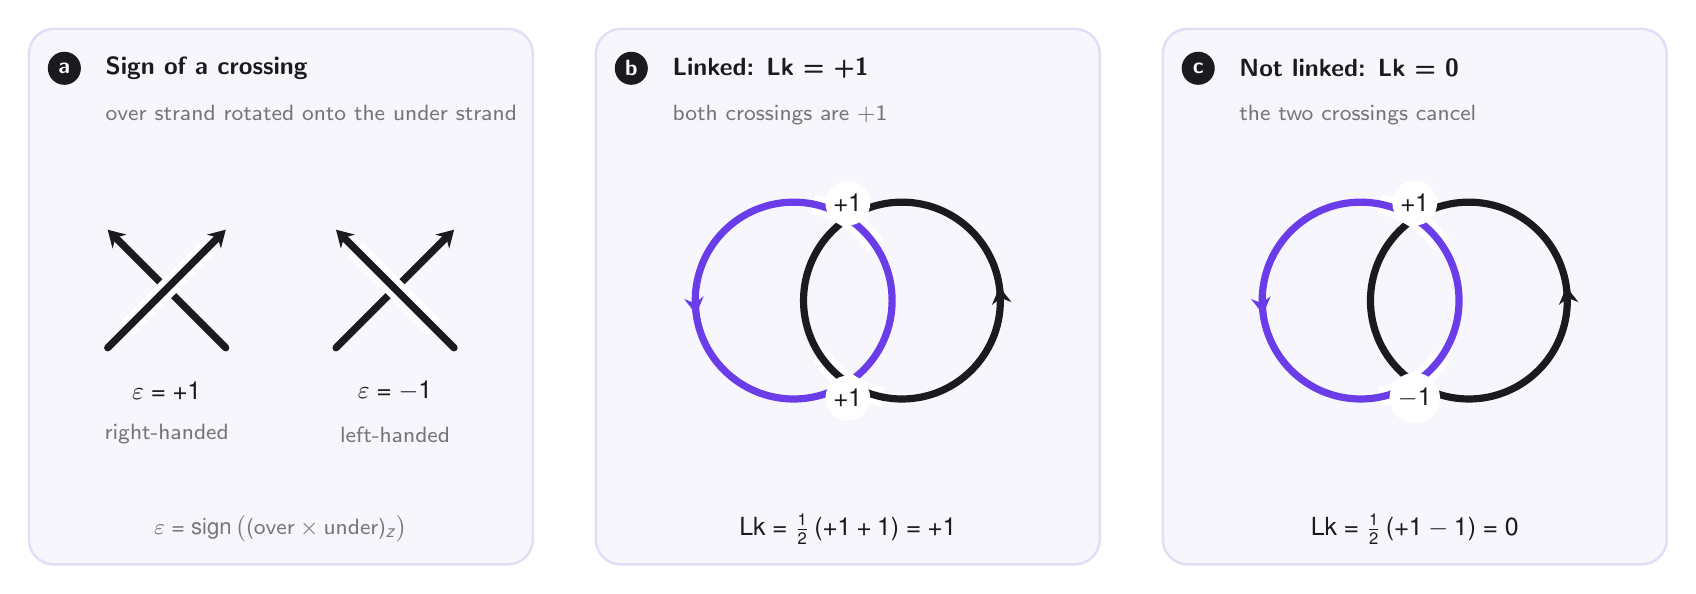
\begin{tikzpicture}
  \foreach \x/\l/\t/\s in {0/a/{Sign of a crossing}/{over strand rotated onto the under strand},7.2/b/{Linked: Lk = +1}/{both crossings are +1},14.4/c/{Not linked: Lk = 0}/{the two crossings cancel}}{
    \panelbg{\x}{-3.2}{\x+6.4}{3.6}\badge{\x+0.45}{3.1}{\l}\node[hd] at (\x+0.85,3.1) {\t};\node[note,anchor=north west] at (\x+0.85,2.75) {\s};}
  % a: the two signs
  \crossing{1.75}{0.3}{p}\crossing{4.65}{0.3}{n}
  \node[lab] at (1.75,-1.0) {$\varepsilon=+1$};\node[lab] at (4.65,-1.0) {$\varepsilon=-1$};
  \node[note] at (1.75,-1.55) {right-handed};\node[note] at (4.65,-1.55) {left-handed};
  \node[note] at (3.2,-2.75) {$\varepsilon=\operatorname{sign}\big((\text{over}\times\text{under})_z\big)$};
  % b: Hopf link, both curves counter-clockwise
  \begin{scope}[shift={(10.4,0.15)},scale=1.25]
    \draw[cA] (-0.55,0) circle (1);\draw[cB] (0.55,0) circle (1);
    \draw[h] ([shift={(-0.55,0)}]34.6:1) arc (34.6:78.6:1);\draw[cA] ([shift={(-0.55,0)}]34.6:1) arc (34.6:78.6:1);
    \draw[h] ([shift={(0.55,0)}]214.6:1) arc (214.6:258.6:1);\draw[cB] ([shift={(0.55,0)}]214.6:1) arc (214.6:258.6:1);
    \draw[cA,-{Stealth[length=6pt,width=7pt]}] ([shift={(-0.55,0)}]182:1) arc (182:188:1);
    \draw[cB,-{Stealth[length=6pt,width=7pt]}] ([shift={(0.55,0)}]2:1) arc (2:8:1);
    \node[lab,fill=white,inner sep=1.5pt,circle] at (0,0.99) {$+1$};\node[lab,fill=white,inner sep=1.5pt,circle] at (0,-0.99) {$+1$};
  \end{scope}
  \node[lab] at (10.4,-2.75) {$\mathrm{Lk}=\tfrac12\,(+1+1)=+1$};
  % c: two overlapping circles, the same curve is over at both crossings
  \begin{scope}[shift={(17.6,0.15)},scale=1.25]
    \draw[cB] (0.55,0) circle (1);
    \draw[h] ([shift={(-0.55,0)}]34.6:1) arc (34.6:78.6:1);\draw[h] ([shift={(-0.55,0)}]-78.6:1) arc (-78.6:-34.6:1);\draw[cA] (-0.55,0) circle (1);
    \draw[cA,-{Stealth[length=6pt,width=7pt]}] ([shift={(-0.55,0)}]182:1) arc (182:188:1);
    \draw[cB,-{Stealth[length=6pt,width=7pt]}] ([shift={(0.55,0)}]2:1) arc (2:8:1);
    \node[lab,fill=white,inner sep=1.5pt,circle] at (0,0.99) {$+1$};\node[lab,fill=white,inner sep=1.5pt,circle] at (0,-0.99) {$-1$};
  \end{scope}
  \node[lab] at (17.6,-2.75) {$\mathrm{Lk}=\tfrac12\,(+1-1)=0$};
\end{tikzpicture}
\end{document}
